% Custom MA template for Rust - Modular game engine
% !TEX encoding = UTF-8 Unicode

% FHTW document class for cooperate identity master thesises
\documentclass[MGS, Master, english]{twbook}
\usepackage[utf8]{inputenc}
\usepackage[T1]{fontenc}

% Define the standard for citations for this paper - IEEE or HARVARD
\newcommand{\FHTWCitationType}{IEEE} 
\ifthenelse{\equal{\FHTWCitationType}{HARVARD}}{\usepackage{harvard}}{\usepackage{bibgerm}}

% Format code listings
\usepackage[final]{listings}
\lstset{captionpos=b, numberbychapter=false,caption=\lstname,frame=single, numbers=left, stepnumber=1, numbersep=2pt, xleftmargin=15pt, framexleftmargin=15pt, numberstyle=\tiny, tabsize=3, columns=fixed, basicstyle={\fontfamily{pcr}\selectfont\footnotesize}, keywordstyle=\bfseries, commentstyle={\color[gray]{0.33}\itshape}, stringstyle=\color[gray]{0.25}, breaklines, breakatwhitespace, breakautoindent}
\lstloadlanguages{[ANSI]C, C++, [gnu]make, gnuplot, Matlab}

% -----------------------------------------
% Format the list of code
\makeatletter
% Setzen der Bezeichnungen für das Quellcodeverzeichnis/Abkürzungsverzeichnis in Abhängigkeit von der eingestellten Sprache
\providecommand\listacroname{}
\@ifclasswith{twbook}{english}
{%
	\renewcommand\lstlistingname{Code}
	\renewcommand\lstlistlistingname{List of Code}
	\renewcommand\listacroname{List of Abbreviations}
}{%
	\renewcommand\lstlistingname{Quellcode}
	\renewcommand\lstlistlistingname{Quellcodeverzeichnis}
	\renewcommand\listacroname{Abkürzungsverzeichnis}
}
% Wenn die Option listof=entryprefix gewählt wurde, Definition des Entyprefixes für das Quellcodeverzeichnis. Definition des Macros listoflolentryname analog zu listoflofentryname und listoflotentryname der KOMA-Klasse
\@ifclasswith{scrbook}{listof=entryprefix}
{%
	\newcommand\listoflolentryname\lstlistingname
}{%
}
\makeatother
\newcommand{\listofcode}{\phantomsection\lstlistoflistings}

% Die nachfolgenden Pakete stellen sonst nicht benötigte Features zur Verfügung
\usepackage{blindtext}

% -----------------------------------------
%
% Einträge für Deckblatt, Kurzfassung, etc.
%
\title{Modular game engine in Rust - Comparing performance and memory usage of subsystems to C++}
\author{Lukas Vogl, BSc.}
\studentnumber{gs16m007}
\supervisor{Dipl.-Ing. Stefan Reinalter}
\secondsupervisor{Mag.rer.nat. Dr.techn. Eugen Jiresch}
\place{Wien}
% German abstract
\kurzfassung{
Modulare Spieleengines zeichnen sich dadurch aus, dass sie intern aus verschiedenen Subsystemen bestehen die unterschiedlichste Aufgaben abarbeiten. Beispielhafte Systeme sind unter anderem Speichermanagement, Rendering oder Physiksimulation. Die Gemeinsamkeit zwischen den Systemen, unabhägig davon wie hardwarenahe oder abstrakt diese sind, sind Aspekte wie Performance und Speicherverbrauch. Um möglichst viel Kontrolle über diese Bereiche zu haben entscheiden sich viele EntwicklerInnen für Systemprogrammiersprachen wie C++ als Entwicklungswerkzeug. Im Zuge dieser Arbeit wird der Autor die seit 2015 existierende Programmiersprache Rust verwenden um ausgewählte Subsysteme einer modularen Spieleengine zu implementieren. Ziel der Arbeit ist es zu untersuchen, ob Rust durch seine neuen Konzepte gängige Schwierigkeiten bei der C++ Entwicklung vermeiden und gleichzeitig eine gleichwertige Performance liefern kann. Dafür werden die in Rust implementierten Systeme zusätzlich in C++ implementiert und anschließend in verschiedenen Szenarien vermessen und verglichen. Aus den Ergebnissen wird evaluiert ob Rust als Programmiersprache für Spieleengines in Frage kommt. Zusätzlich werden die Implementierungsdetails der verschiedenen Sprachen und Systeme behandelt, wodruch aufgezeigt wird welche Unterschiede zwischen den beiden Sprachen bestehen.

}
\schlagworte{Rust, C++, Engine, Speichermanagement, Performance}
% English abstract
\outline{
Modular game engines are defined by the fact that they are composed of different subsystems working on many distinct tasks.
Exemplary systems are, inter alia, memory management, rendering or physics simulation. The similarity between the systems, regardless of how low-level or abstract they are, are performance and memory consumption. To gain control over these fields most programmers choose system programming languages such as C++ as development tool. In this thesis the the author chose the programming language Rust to implement selected subsystems of a modular game engine. Is it the goal of the thesis to investigate whether Rust can avoid common difficulties known from C++ due to its new concepts while maintaining C++ like performance. For this purpose the selected systems will also be implemented in C++. They are then surveyed in different scenarios and compared to each other. The results are evaluated to see whether it is worth considering using Rust as a language for game engine programming. Furthermore the implementation details ofthe different languages and systems are discussed whereby the differences between the two languages are outlined;
}
\keywords{Rust, C++, Engine, Memory management, performance}
\acknowledgements{\blindtext}

% -----------------------------------------
\begin{document}
	
%Festlegungen für den HARVARD-Zitierstandard
\ifthenelse{\equal{\FHTWCitationType}{HARVARD}}{
	\bibliographystyle{Harvard_FHTW_MR}%Zitierstandard FH Technikum Wien, Studiengang Mechatronik/Robotik, Version 1.2e
	\citationstyle{dcu}%Correct citation-style (Harvardand, ";" between citations, "," between author and year)
	\citationmode{abbr}%use "et al." with first citation
	\iflanguage{ngerman}{
		%Deutsch Neue Rechtschreibung
		\newcommand{\citepic}[1]{(Quelle: \protect\cite{#1})}%Zitat: Bild
		\newcommand{\citefig}[2]{(Quelle: \protect\cite{#1}, S. #2)}%Zitat: Bild aus Dokument
		\newcommand{\citefigm}[2]{(Quelle: modifiziert "ubernommen aus \protect\cite{#1}, S. #2)}%Zitat: modifiziertes Bild aus Dokument
		\newcommand{\citep}{\citeasnoun}%In-Line Zitiat entweder mit \citep{} oder \citeasnoun{}
		\newcommand{\acessedthrough}{Verf{\"u}gbar unter:}%Für URL-Angabe
		\newcommand{\acessedthroughp}{Verf{\"u}gbar bei:}%Für URL-Angabe (Geschützte Datenbank, Zugriff durch FH)
		\newcommand{\acessedat}{Zugang am}%Für URL-Datum-Angabe
		\newcommand{\singlepage}{S.}%Für Seitenangabe (einzelne Seite)
		\newcommand{\multiplepages}{S.}%Für Seitenangabe (mehrere Seiten)
		\newcommand{\chapternr}{K.}%Für Kapitelangabe
		\renewcommand{\harvardand}{\&}%Harvardand in Zitaten
		\newcommand{\abstractonly}{ausschließlich Abstract}
		\newcommand{\edition}{. Auflage}%Angabe der Auflage
	}{
		\iflanguage{german}{
			%Deutsch
			\newcommand{\citepic}[1]{(Quelle: \protect\cite{#1})}%Zitat: Bild
			\newcommand{\citefig}[2]{(Quelle: \protect\cite{#1}, S. #2)}%Zitat: Bild aus Dokument
			\newcommand{\citefigm}[2]{(Quelle: modifiziert "ubernommen aus \protect\cite{#1}, S. #2)}%Zitat: modifiziertes Bild aus Dokument
			\newcommand{\citep}{\citeasnoun}%In-Line Zitiat entweder mit \citep{} oder \citeasnoun{}
			\newcommand{\acessedthrough}{Verf{\"u}gbar unter:}%Für URL-Angabe
			\newcommand{\acessedthroughp}{Verf{\"u}gbar bei:}%Für URL-Angabe (Geschützte Datenbank, Zugriff durch FH)
			\newcommand{\acessedat}{Zugang am}%Für URL-Datum-Angabe
			\newcommand{\singlepage}{S.}%Für Seitenangabe (einzelne Seite)
			\newcommand{\multiplepages}{S.}%Für Seitenangabe (mehrere Seiten)
			\newcommand{\chapternr}{K.}%Für Kapitelangabe
			\renewcommand{\harvardand}{\&}%Harvardand in Zitaten
			\newcommand{\abstractonly}{ausschließlich Abstract}
			\newcommand{\edition}{. Auflage}%Angabe der Auflage
		}{
			%Englisch
			\newcommand{\citepic}[1]{(Source: \protect\cite{#1})}%Zitat: Bild
			\newcommand{\citefig}[2]{(Source: \protect\cite{#1}, p. #2)}%Zitat: Bild aus Dokument
			\newcommand{\citefigm}[2]{(Source: taken with modification from \protect\cite{#1}, p. #2)}%Zitat: modifiziertes Bild aus Dokument
			\newcommand{\citep}{\citeasnoun}%In-Line Zitiat entweder mit \citep{} oder \citeasnoun{}
			\newcommand{\acessedthrough}{Available at:}%Für URL-Angabe
			\newcommand{\acessedthroughp}{Available through:}%Für URL-Angabe (Geschützte Datenbank, Zugriff durch FH)
			\newcommand{\acessedat}{Accessed}%Für URL-Datum-Angabe
			\newcommand{\singlepage}{p.}%Für Seitenangabe (einzelne Seite)
			\newcommand{\multiplepages}{pp.}%Für Seitenangabe (mehrere Seiten)
			\newcommand{\chapternr}{Ch.}%Für Kapitelangabe
			\renewcommand{\harvardand}{\&}%Harvardand in Zitaten
			\newcommand{\abstractonly}{Abstract only}
			\newcommand{\edition}{~edition}%Edition -> note, that you have to write "edition = {2nd},"!
}}}

\maketitle

\chapter{Introduction}
Game engines are an essential part of the gaming industry. Todays state-of-the-art game engines have committed themselves to the goal of creating visually appealing games while providing reasonable performance. Achieving this requires the engine engineers to invest a great amount of time and know-how of underlying hardware. Many of these engines, choosing Unity and Unreal Engine 4 as example, are using C++ as underlying technology. C++ is the language of choice due to it's capabilities of managing memory manually without the limitations of a garbage collector. These capabilities are the foundation for high performance software and essential to game engines. But while the benefits of manual memory management are indisputable it also comes with common pitfalls. 

This thesis aims to examine whether the system programming language Rust can be used as a replacement for C++. Rust claims to avoid pitfalls made in C++ while maintaining similar performance. As a basis for discussion the author will implement selected engine subsystems: memory management, containers and an \ac{ECS}. All systems, except for the \ac{ECS} which already exists in Rust, are written in Rust and C++ to later measure and compare their performance in different scenarios. The results of the measurements shall then serve as the basis for the discussion if Rust can be considered as a viable language for game engine programming.

Chapter 2 will introduce the reader to the history and evolution of game engines. It will also outline state-of-the-art products and shortly describe them. In chapter 3 important tools that are tightly related to the underlying engine and the concept of an asset pipeline are discussed, concluding the chapter with a section presenting the theory and examples of selected engine subsystems.
The next chapter provides the reader with an overview of the Rust programming language. It describes the current state of Rust and creates a basic understanding of it by introducing the most important concepts and patterns. It will then compare common and well-known C++ problems and pitfalls with corresponding code in Rust. At the end the author outlines encountered difficulties that can occur when working with Rust. 
In chapter 5 the author talks about the implementation details of the implemented subsystems and where the differences between Rust and C++ are visible. The development process, architecture and project setup of the Spark engine (the implemented submodules will serve as a basis for this engine in future work) will be discussed. The performance measurement results and observed scenarios are then compared and discussed in chapter 6. Chapter 7 will then finish the thesis with the conclusion.

% Game engine arch
\chapter{Game engines}

Game engines are tightly connected to the evolution of video games themselves. Where 50 years ago a game was build out of hardware the rapid development of a computer's processing power and storage capabilities changed the process of how games are made. Today a game runs on machines assembled from multiple cores, several \acp{GB} of \ac{RAM} and a powerful \ac{GPU}. But whether the target platform is a PC or a specialized gaming console every modern game has to fulfill certain constraints to be a viable product. This chapter will highlight some of the most important milestones in the history of video games and game engines. It will also give an overview of well-known products on the game engine market and will conclude with the description of selected submodules, the underlying building blocks of a game engine.

\section{Evolution of game engines}

When the first developers started to create video games, the term \textit{game engine} was non existent. At this time the software that ran the simulation a player experienced was tailored to the needs of a specific genre, hardware and game. It was then in the 1990s and with the rise of games like \textit{Doom (1993)} and \textit{Quake (1996)} that certain software was referred to as a \textit{game engine}. The mentioned games separated their technical backbones into different components, creating an architecture that distinguishes between core software modules and game specific entities such as art assets, levels and the general rules of the game. Due to the well-designed architecture and separations the effort to create a new game, where the general concept is the same, was reduced from writing every system and piece of code to creating new art and only tweak and configure the software of previous games. This was also the birth of the \textit{modding} community, where individuals and also studios modify existing games or engine software to create new content or whole games.

From that time on the developers created their games with modding and future extension in mind. Smaller studios started to license parts of the engine software they could not afford to create by themselves, be it money, time or man power. With the concept of licensing, studios, that built the extensible and reusable software packages, created another source of income. But while the goal of an extensible and reusable software collection is a desirable one, the line between a game and an engine is often softer than desired. Because of the games nature and their specific genre rules, it is hard, if not even impossible, to develop a generic engine that can serve as a template for every game. It became the responsibility of engine developers to find the balance between general-purpose functionality and game or platform tailored optimizations. This trade-off has to be made because the developer can only assume how the software will be used. And so a game engine developed and optimized for rendering \acp{FPS} will probably not run a \ac{RTS} game with maximum performance due to the different rule sets and features both genres require.

Empowered by the wish of creating games that can be modified and licensed, bigger studios started to create commercial engines. \textit{Id Software}, the company that created \textit{Doom} and the \textit{Quake} trilogy, opened up the field with their \ac{FPS} engines in the early 1990s. \textit{Id Software} was then followed by \textit{Epic Games, Inc.}, creator of the Unreal Engine, which powered their well-known game \textit{Unreal} and later the \textit{Unreal Tournament} series. The current version, the \ac{UE4}, is one of the most popular game engines of our time and will be described in the next section. Other game engines released in the same period and which should not be left unmentioned are \textit{CryENGINE} (Crytech), \textit{Source Engine} (Valve), \textit{Frostbite} (DICE) and \textit{Unity}.

For a long time many of the mentioned engines, if not all, followed a model of selling licenses to developers for accessing the engine and its source code. But it was around 2009 and again in 2015 that big engine developers, including Unity and Epic Games, decided to rework their business model and let developers use their software for free. The license terms often include a revenue share if the game should be successful but the basic usage of the engine is free most of the time. Although this certainly had a huge impact on smaller products and teams, that could not compete with the teams working at Epic or Unity, this decision lowered the entrance barrier for game developers and students. This transition to accessible license models and free access can be seen as one of the biggest milestones in the modern history of game engines.

Speaking of Unity and Epic, the next section will describe modern game engines on the market, how they work and what they are used for. In contrast to Unity and \acl{UE4}, two smaller engines will be described to show the difference between approaches and why the flexibility of smaller engines and teams can also be an advantage over big software projects.


\section{Modern commercial game engines}

As described in the previous section game engines evolved from extensible game or genre tailored software to standalone viable products used to create different games. The market is actually dominated by two big engines, Unity and Unreal Engine 4, whereas the rest is separated between custom in-house and several medium to small engines and open source projects. The author is going to describe the features and license models of the two big solutions as well as of two smaller but more flexible ones.

\subsection{Unreal Engine 4}

As already known \textit{Epic Games, Inc.} released the first version of the Unreal Engine with their game \textit{Unreal}. The solution was quickly adopted and Epic developed two more generations, Unreal Engine 2 and 3, before the current generation, called \ac{UE4}, was released. 
All generations powered well-known games such as Deus Ex (UE1), Tom Clancy’s Splinter Cell: Pandora Tomorrow (UE2), Gears of War (UE3) or Fortnite (UE4), to name a few.

While previous generations could be licensed by developers for a license fee, Epic first changed their licensing model to a monthly fee and later lowered the access barrier even more by getting rid of any license fee at all. The current version of \ac{UE4} is for free and source code access can be requested at GitHub (https://github.com/EpicGames/UnrealEngine). This move allowed many developers to create their projects with \ac{UE4} and Epic is eligible for a 5\% share if the game makes more than 3000\$ per calendar quarter in revenue.

When working with \ac{UE4} the developer can choose to build everything from source or work with distributed pre-built binaries. Due to the fact that the Unreal family of engines was developed with first- and third person shooters in mind, the source code access is often appreciated by developers to tweak and rework the engine in a way to better run games from other genres. Regardless whether the engine was built from source or not, when working with it the user interacts with the integrated editor, often also referred to as \textit{UnrealEd}. It is the entry point to nearly every tool that ships with \ac{U4}.

\begin{figure}[h!]
	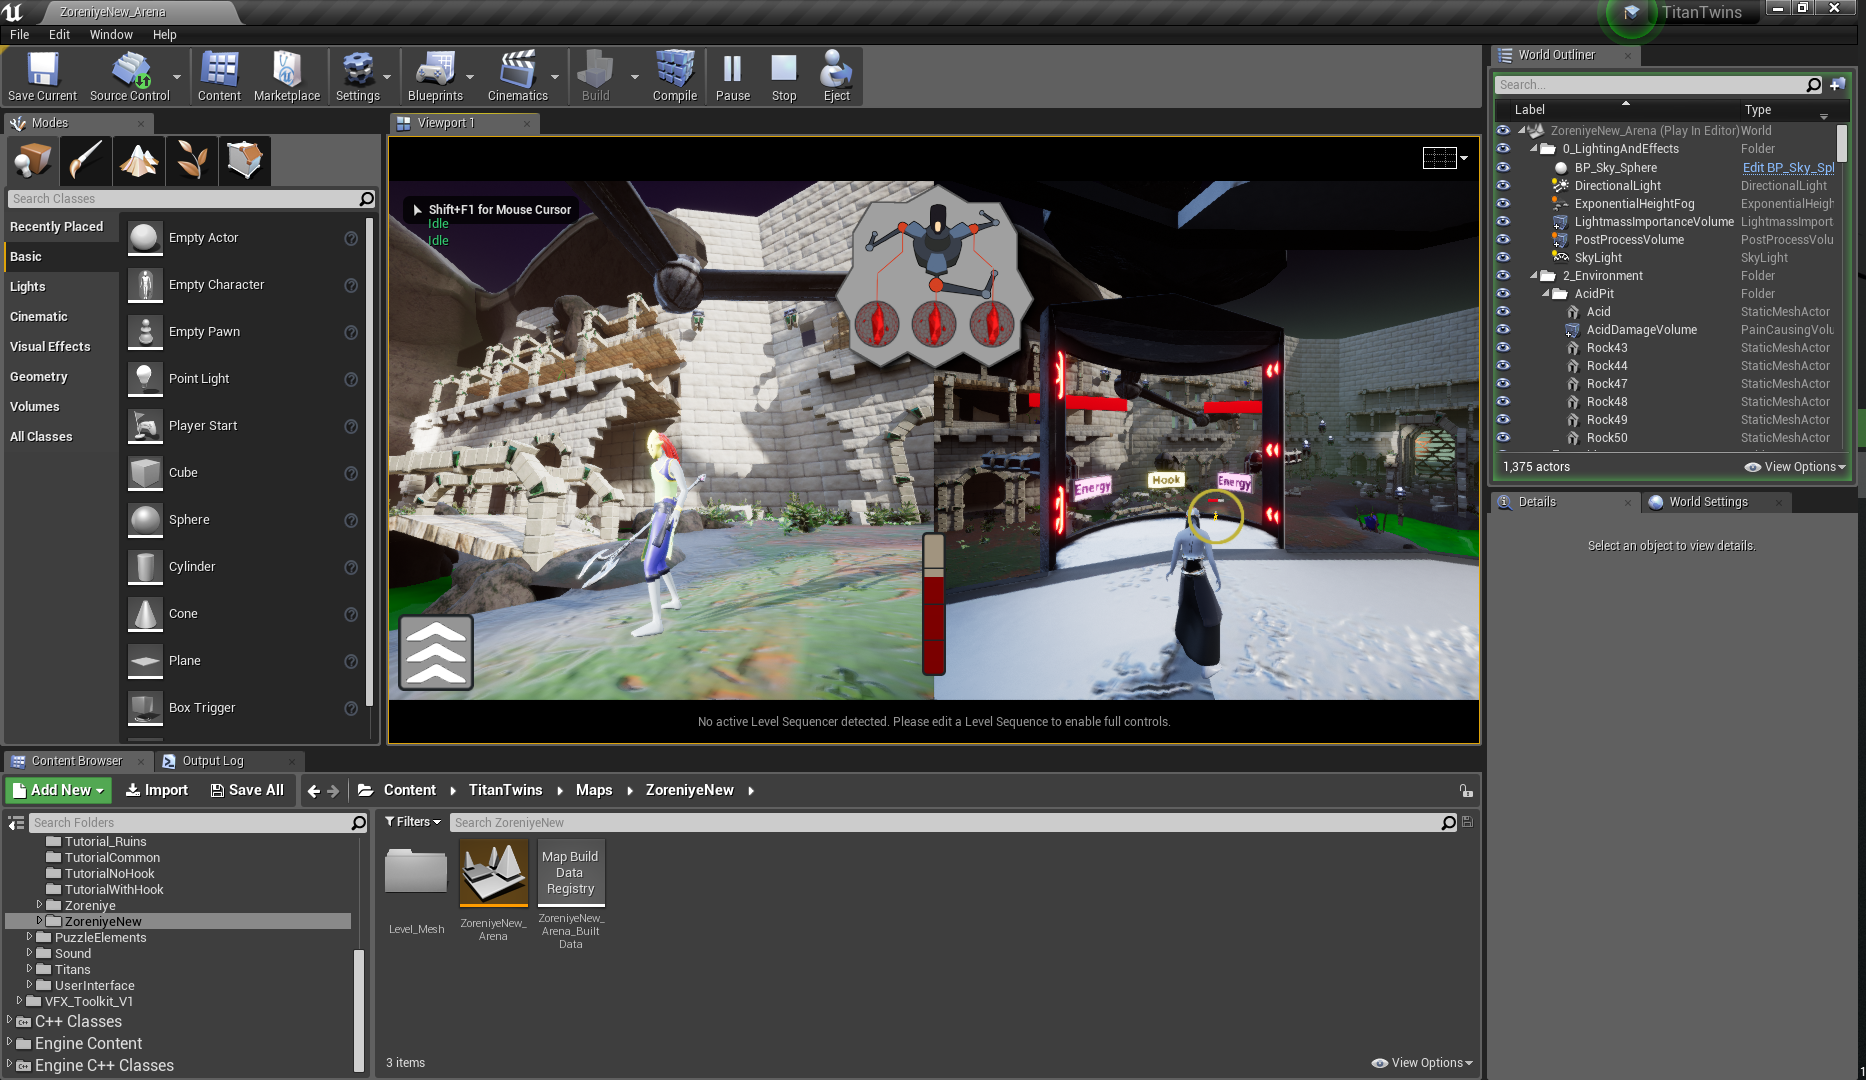
\includegraphics[width=\linewidth]{PICs/unreal_ed.png}
	\caption{The editor shipped with \ac{UE4}}
	\label{fig:unreal_ed}
\end{figure}

Going from left to right and top to bottom, Figure \ref{fig:unreal_ed} shows a selection for actors (objects that can be placed in the game world), a game world view, the world outliner (hierarchy of actors) and the content browser, that lists all folders and contained assets. The editor is a place where designers can create the game world, where artists can author special effects and their assets directly in the game
and where designers and programmers can develop the rules and logic needed to drive the world. For creating this logic \ac{UE4} offers two possible ways: scripting via the \textit{Blueprint} system or directly in C++. \ac{UE4} comes with the integrated \textit{Blueprint Visual Scripting} system that allows for gameplay programming using the concept of a node-based graph. This system is versatile and if it has reached it's capacities a programmer can still implemented the necessary or performance critical parts in C++ and expose an interface for the designer to use the component together with built-in blueprints.

\begin{figure}[h!]
	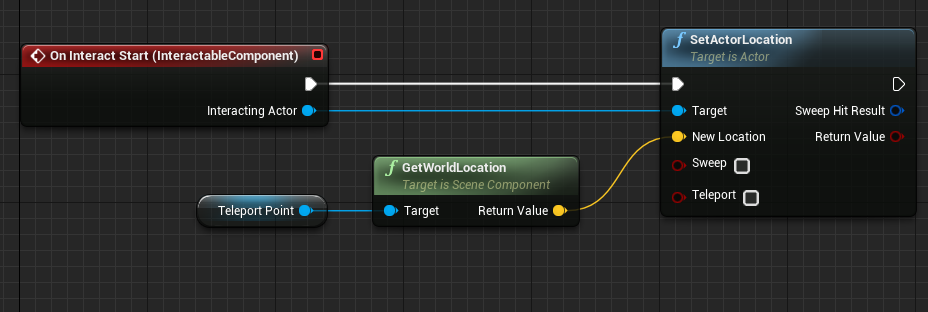
\includegraphics[width=\linewidth]{PICs/ue_blueprints.png}
	\caption{A very simple example that shows how the blueprint visual scripting looks like in \ac{UE4}}
	\label{fig:ue_blueprints}
\end{figure}

A very similar system of node-based graphs is used for building complex materials in \ac{UE4}. A material describes how an object, that uses it, looks like. It can for example define how it reacts upon light, whether the object appears to be rough or specular. The advantage of \ac{UE4}'s approach, using a node-based abstraction for materials, is that it makes life easier for developers when creating and authoring styles or effects. Without this system in place it would require a graphics programmer to write a shader. There are many different kinds of shaders but to keep it simple and because it is not necessary for now it is enough to say that a shader is a program that is executed on the \ac{GPU} and defines which color a pixel shall display at the end. Writing such shaders is not a trivial task. The node-based approach puts a layer of abstraction upon this process that allows developers to work with materials without needing to know the low-level internals of shaders.

It should not be unmentioned that working with \ac{UE4}, especially when needing very specific features or techniques that are not exposed to the abstraction systems, it requires a fond knowledge of C++ and the internal engine systems to fulfill the task. \ac{UE4} has grown in the past years and due to the fact that its source code is authored by many developers, both Epic engineers and open source contributors, bug reports are likely prioritized in relation to the needs Epic has for its own products developed in \ac{UE4}. The documentation is well written for engine tools and visual scripting but is a little weak on the C++ side. When working directly in C++ sometimes compile-times can decrease iteration times in \ac{UE4} which is due to the \ac{UBT} and some default configurations on how to deal with precompiled headers and unity builds.

To conclude this paragraph about \ac{UE4} it can be said that Epic created an engine that is suitable for creating games from any genre, which sometimes require tweaking the engine's source code. \ac{UE4} offers a variety of tools and integrations for asset authoring software which makes it easy for developers to start working with it. The abstraction systems paired with the revenue share licensing model lowered the entrance barrier for new game developers and are a reason for why the engine is in such a good market position. The development experience and fast iteration times fade away the more direct C++ coding is involved but again a trade-off between developing every system in-house and dealing with problems that rise has to be made.

\subsection{Unity}

The biggest competitor on the market for \ac{UE4} is Unity, and there are several reasons why there is a second product that viable. Unity was born in 2004 and created by the company called \textit{Over the Edge} which was later re-branded to \textit{Unity Technologies}. Contrary to the evolution of \ac{UE4} that evolved from moddable games and with easy extension in mind, Unity was created to lower the access barriers for 2D and 3D game development. After their first game, GooBall, failed commercially the founders discovered how valuable engine software and tools are. This led to their decision of building an engine that is accessible to as many people as possible and that promises ease of development and cross-platform support. With these principles in mind Unity became a product that was adopted by many developers and nowadays is used by many studios and small developers.

In contrast to \ac{UE4} the source code of Unity is not freely accessible but it can be acquired by acquiring an enterprise subscription. If source code access is not needed, which is the case more a major percentage of the developer products, Unity offers a very fair licensing model. A personal license can be registered for free, with the constraint that a product does not generate more revenue than 100.000\$ annually. This version includes all Unity core features as well as continuous upgrades and access to Unity beta versions. The next tier, called Unity Plus, includes everything of the previous one and adds more flexible customizations (custom splash screen, pro editor UI), more in depth analytics and it alters the cap of concurrent players on multiplayer games hosted by Unity. The Plus tier costs 35\$ per month and is constrained by a revenue cap of 200.000\$ per year. If the income exceeds that limit, the Unity Pro tier comes without any revenue limit at all for 125\$ per month. It adds again more in-depth analytics and alters the concurrent players cap once more. Independent of the selected tier, Unity includes an editor to interact with its tools and the game world. 

\clearpage

\begin{figure}[h!]
	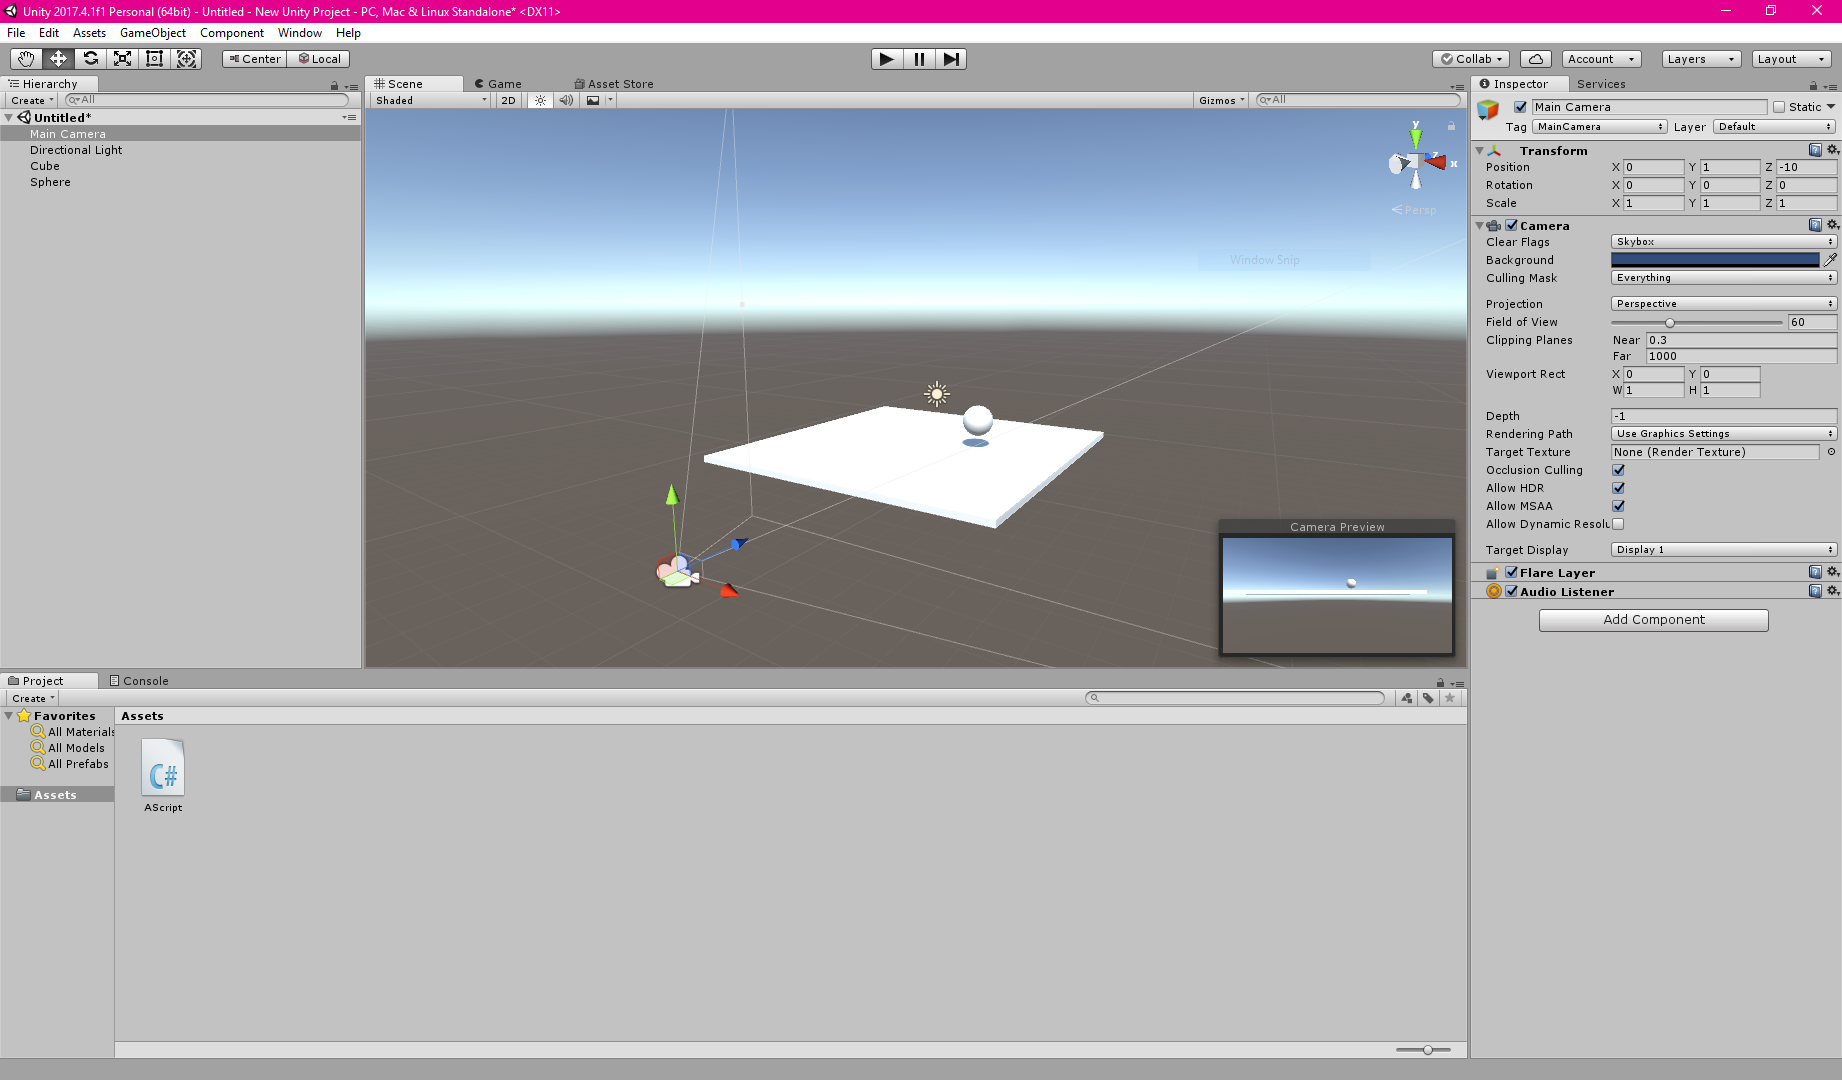
\includegraphics[width=\linewidth]{PICs/unity_ed.png}
	\caption{The default layout of the editor shipped with Unity}
	\label{fig:unity_ed}
\end{figure}

The editor is quite similar to the one of \ac{UE4} but the views and tools differ in their naming. Going from left to right and top to bottom Figure \ref{fig:unity_ed} shows the Hierarchy, collection of game objects that are placed in the game world, the scene or current world, the Inspector, a list of components attached to a single game object and the project structure showing folders and assets. 
What was called an actor in \ac{UE4} can be compared to a game object in Unity. A game object is an entity that can be placed in the world but does not contain any logic itself. Rather it is a container that holds a collection of components, each holding data or logic. This system of entities and components is called an \acl{ECS} and will be described in detail at the end of this chapter. Because of the \ac{ECS} components can be shared and reused among projects which simplifies the development process and cuts iteration times when done properly.
It was already mentioned that components can also contain logic which already describes the basics on how game rules and logic are created in Unity. Where \ac{UE4} provides a visual scripting system Unity does not have anything similar. In Unity scripting is done in C\#, a high-level programming language running in the MonoDevelop/.Net runtime. The work flow of creating gameplay logic often starts with a programmer creating a new scripting component in C\# which then later can be used by designers to assemble new game objects without needing to touch any C\# code. This is ensured by a system that allows programmers to expose certain properties of the script to the editor, where values can be tweaked by designers to fit the needs of the game. Although Unity does not have a visual scripting system it is easy to create and run scripts because they are contained withing a single component and an error inside of them will not crash the whole engine but is guarded by the scripting runtime.

\clearpage

\begin{lstlisting}[language={[Sharp]C}, frame=single, caption={Example of an empty C\# script in Unity}, label={Script}]
using System.Collections;
using System.Collections.Generic;
using UnityEngine;

public class AScript : MonoBehaviour {
	// Use this for initialization
	void Start () {
	// Execute code at component start ...
	}
	
	// Update is called once per frame
	void Update () {
	// Execute code once per frame ...
	}
}
\end{lstlisting}

While previous versions of Unity supported two additional scripting languages, Boo and Javascript, C\# was the most dominant scripting language used among Unity games. 

A long time it was the node-based material graph that separated Unity and \ac{UE4}, but since version 2018.1 (that is in beta-state at the time of writing) Unity introduces the \textit{Shader Graph}, seen in Figure \ref{fig:unity_shader_graph}, which serves as a visual interface for building shaders. Together with the \textit{Scriptable Render Pipeline} and the new job system, programmers gain more access over low-level and performance critical parts of the engine which closes the gap to \ac{UE4} a bit more regarding performance and control.

\begin{figure}[h!]
	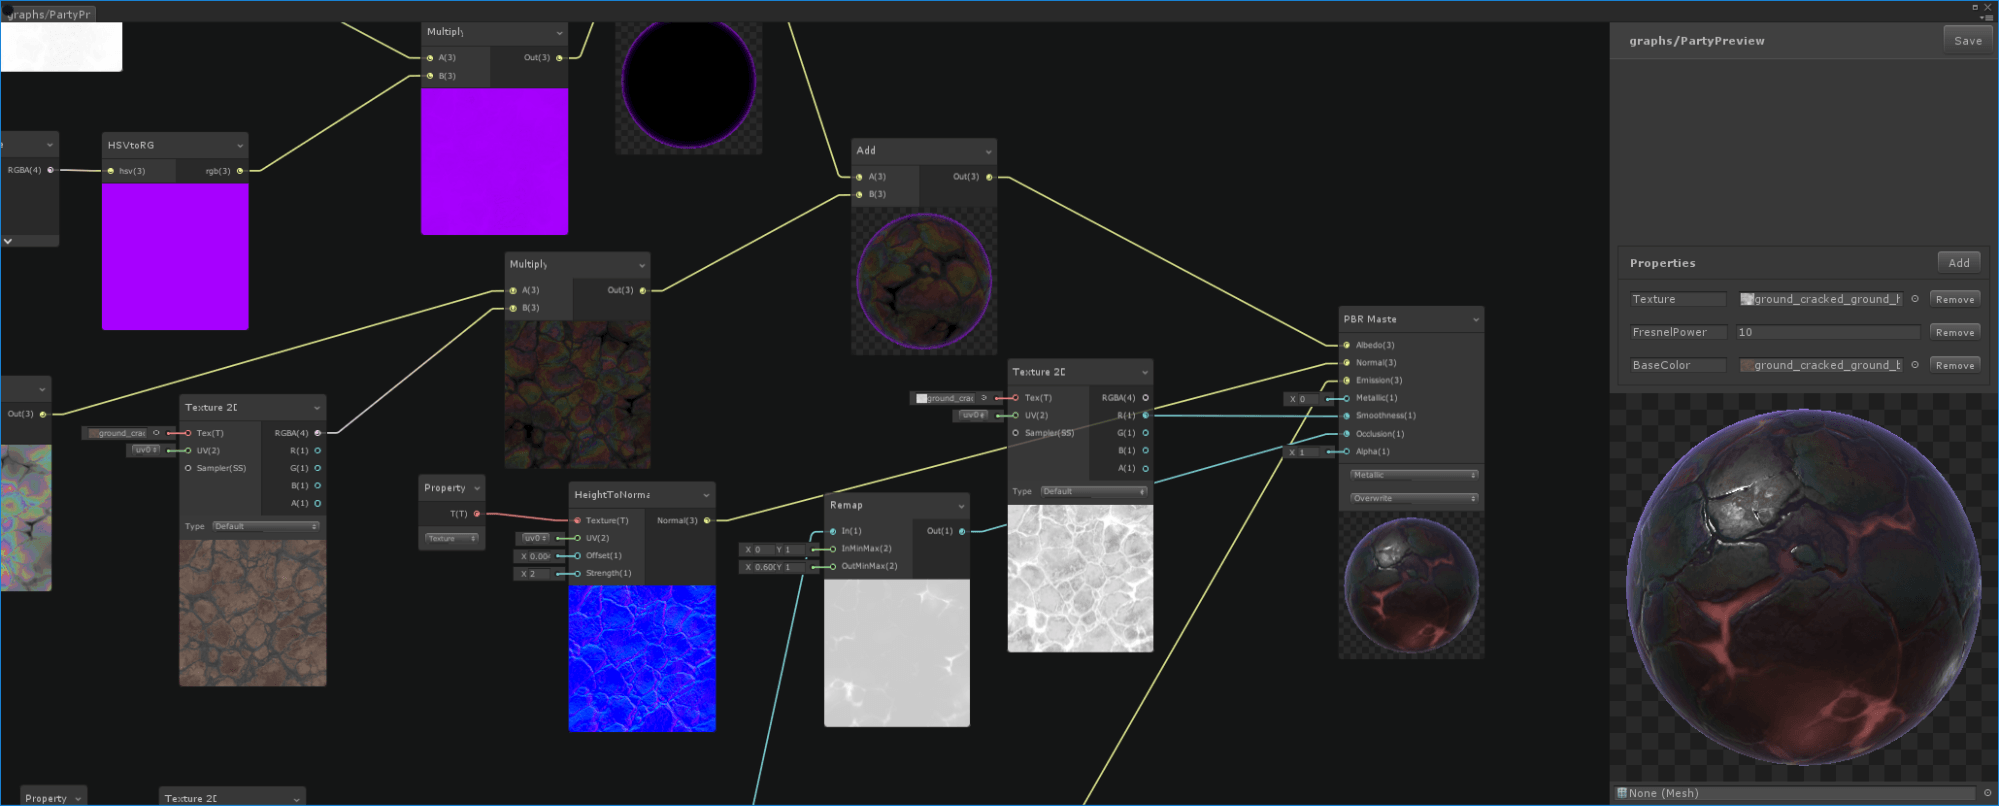
\includegraphics[width=\linewidth]{PICs/unity_shader_graph.png}
	\caption{The new visual shader graph editor that ships with Unity 2018.1}
	\label{fig:unity_shader_graph}
\end{figure}

Together with all these features and the asset store, a marketplace hosted by Unity where developers can upload, download and sell components, art and different plugins Unity is a tool suitable for games from any genre. Its low entrance barriers and support for many different platforms make it a powerful competitor to \ac{UE4}. It is also due to these aspects that Unity is the tool of choice for game developers that plan to release on mobile platforms, such as Android or IOS. Unity is also the engine often chosen for rapid prototyping due to good iteration times and the asset store.

\subsection{Molecular}
\blindtext

\subsection{Tombstone}

The Tombstone engine is developed by \textit{Terathon Software}, which was founded by Eric Lengyel in 2001. It is a cross-platform engine written in C++ that runs on Windows, Playstation 4, Linux and MacOS. This engine is mentioned in this chapter because it features an interesting architecture and invented and uses several innovative and robust techniques.
The Tombstones engine architecture is separated into several layers of managers combined with general utility libraries and a plugin system. General utilities such as memory management and a container library build the bases for managers of different systems. These system manager include for example the resource, thread and graphics manager. Upon this layer more high level managers are built that handle the game world, the scene hierarchy or the animation system. To work with these systems Tombstone offers several plugins, shipped with the engine.

 \begin{figure}[h!]
 	\centering 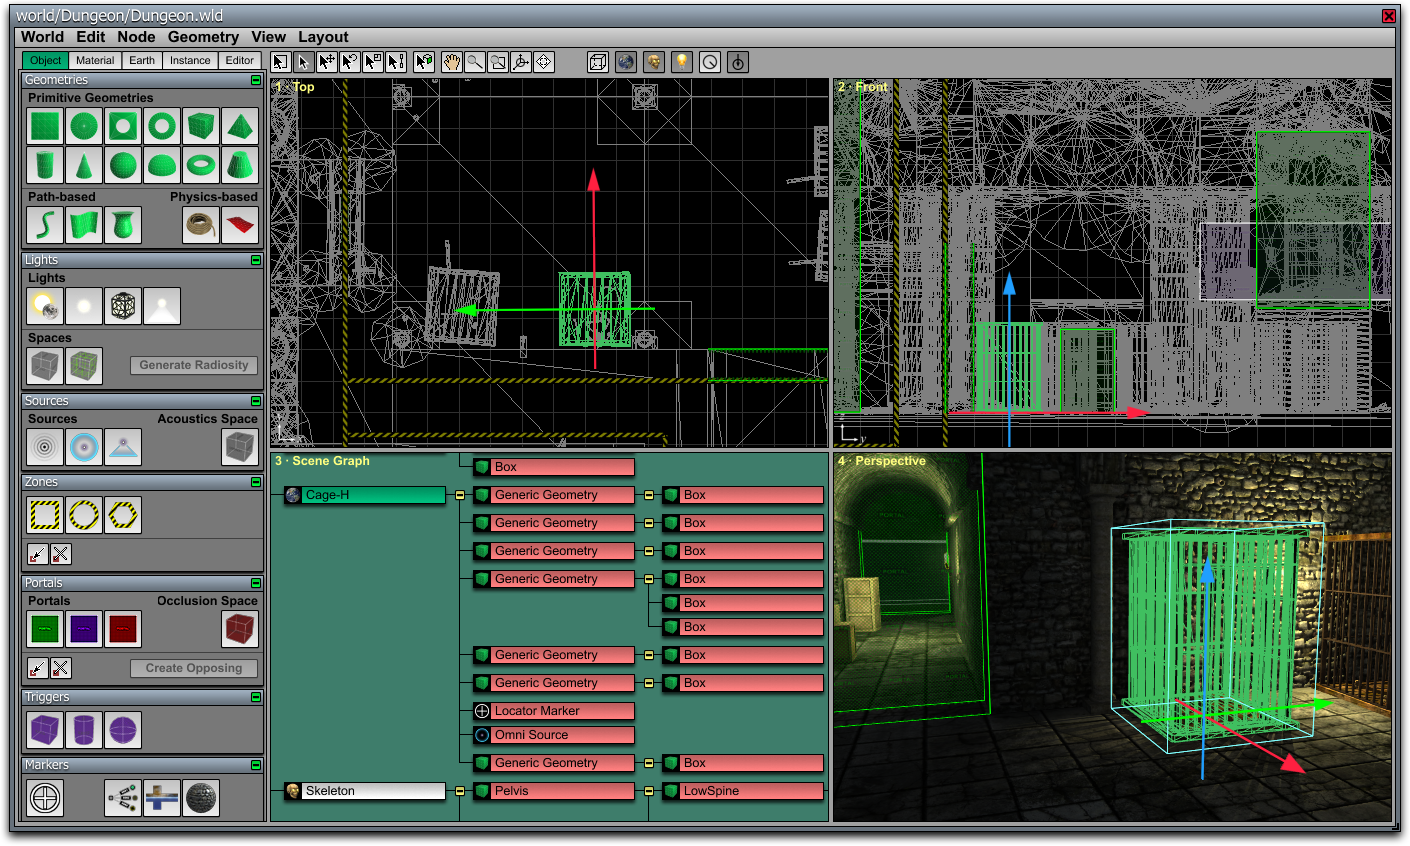
\includegraphics[width=0.5 \linewidth]{PICs/tombstone_ed.png}
 	\caption{The world editor plugin used to edit worlds in the Tombstone engine}
 	\label{fig:tombstone_ed}
 \end{figure}

Among these there is also the world editor that, similar to the bigger engines, allows for creating worlds and levels. Beside the world editor other plugins are a visual shader editor, several tools for importing assets and \ac{UI} builder to generate panels and widgets. Beside the well-defined architecture Tombstone features two standards also created by Eric Lengyel, named the \ac{OpenDDL} and the \ac{OpenGEX}. These protocols are used for exchanging data with asset authoring software like Maya or Photoshop and to store serialized data. The design of the architecture if very well described in a visual form directly at the Tombstone homepage (http://tombstoneengine.com/architecture.php).

Contrary to the bigger companies the Tombstone engine's licensing model does not offer free versions. To acquire a lifetime license for all platforms (Windows, Linux \& MacOS) a fee of 495\$ per person has to be paid. This license does not include any revenue share nor is it limited to a specific amount of shipped games.

The Tombstone engine is an example of a quality piece of software and showcases in what direction an engine can develop if the design goals are carefully thought out. It also tries to establish open standards for exchanging data between different parts of the game development toolchain. If such standards would be implemented and obeyed by more engines it would ease the process of migrating the workflow of engineering teams to another engine or software that would better fit their current project.

\section{Rust game engines}

Because the goal of this thesis is to research whether Rust is a potential choice for a game engine's main language, the author wants to highlight work already done in that field. All previously described solutions are driven by C++. While some of them use it for the entire engine, others built only their core systems in C++ and use higher level languages on top of it. To showcase what was already done in the Rust ecosystem and to better understand some decisions the author made when implementing the submodules, this section is dedicated to the two biggest engines written in Rust - Piston and Amethyst.

\subsection{Piston}

Piston is a modular game engine written in Rust that is now maintained as an open source project on GitHub. It was created in 2014 byt developer Sven Nilsen. Having been a testing field for 2D graphics in Rust, working with different back-ends, the project evolved into what is called Piston today. The engine is separated into different modules, each handling a specific task. The contributors are currently developing solutions for 2D and 3D rendering, window management, plugins for \acp{IDE} like Visual studio and other systems connected to games. The Piston project aims to generate an ecosystem that reduces development cost for games. Due to this desire the functionality is separated into the distinct modules to allow them to be reused between multiple projects. Contrary to Unity or \ac{UE4} Piston does not include any editor to work directly in the 3D or 2D world. It is up to the developer of a game or an open source contributor to implement such a tool, that can be put on top of the already existent ecosystem libraries.

\subsection{Amethyst}

The second engine commonly mentioned in the Rust ecosystem in Amethyst. It is a data-oriented game engine written in Rust. On the project page the developers describe that Amethyst is inspired by the \textit{Bitsquid Engine}, that is now called \textit{Autodesk Stingray}. Being inspired by the Bitsquid the engine's goal include a parallel architecture featuring an \ac{ECS} and an optimized renderer using modern \acp{API} such as Vulkan or Direct3D 12 and greater. On the tool side it plans to split the commonly known world editor into several distinct tools, but at the moment just a single tool, used for creating and deploying projects, is implemented.. Just as Piston, Amethyst is an open source project under the MIT/Apache2 license that is hosted and maintained at GitHub.

Due to the infancy of both projects and the language in general neither Piston nor Amethyst can be compared to commercial engines like Unity or \ac{UE4}. But these projects create a fond basis for game development in Rust and both already built a strong community that is eager to push the boundaries of Rust.
\chapter{Engine architecture overview}

Now, after the last chapter described many different kinds and sizes of engines, this section is going to examine the architecture that powers an engine. At the beginning an overview of a modern game engine's runtime architecture is given. That overview is then followed by a description of several selected submodules. These power different systems of the engine and are responsible for its performance and functionality. The submodules were chosen based on the author's opinion of their relevance and importance to the backbone of an engine.

\section{General runtime architecture}

When talking about software parts of an engine in a high level fashion it can be separated into two clearly diverging parts, tools and the runtime component. This section will almost entirely discuss the runtime part while only mentioning the most important tools at the end. An engine consists from many modules which are separated into different layers. Game engines share this architectural design decision with many other software projects that reach a specific size. Layers group modules together with other ones operating in the same order of magnitude as their siblings. A layer often depends upon lower ones but shall not have any dependencies to upper ones. This ensures that coupling between layers is loose which leads to more stable software solutions. An exemplary illustration of a generic engine's runtime architecture can be seen in Figure \ref{fig:engine_runtime_arch}.

\begin{figure}[h!]
	\centering 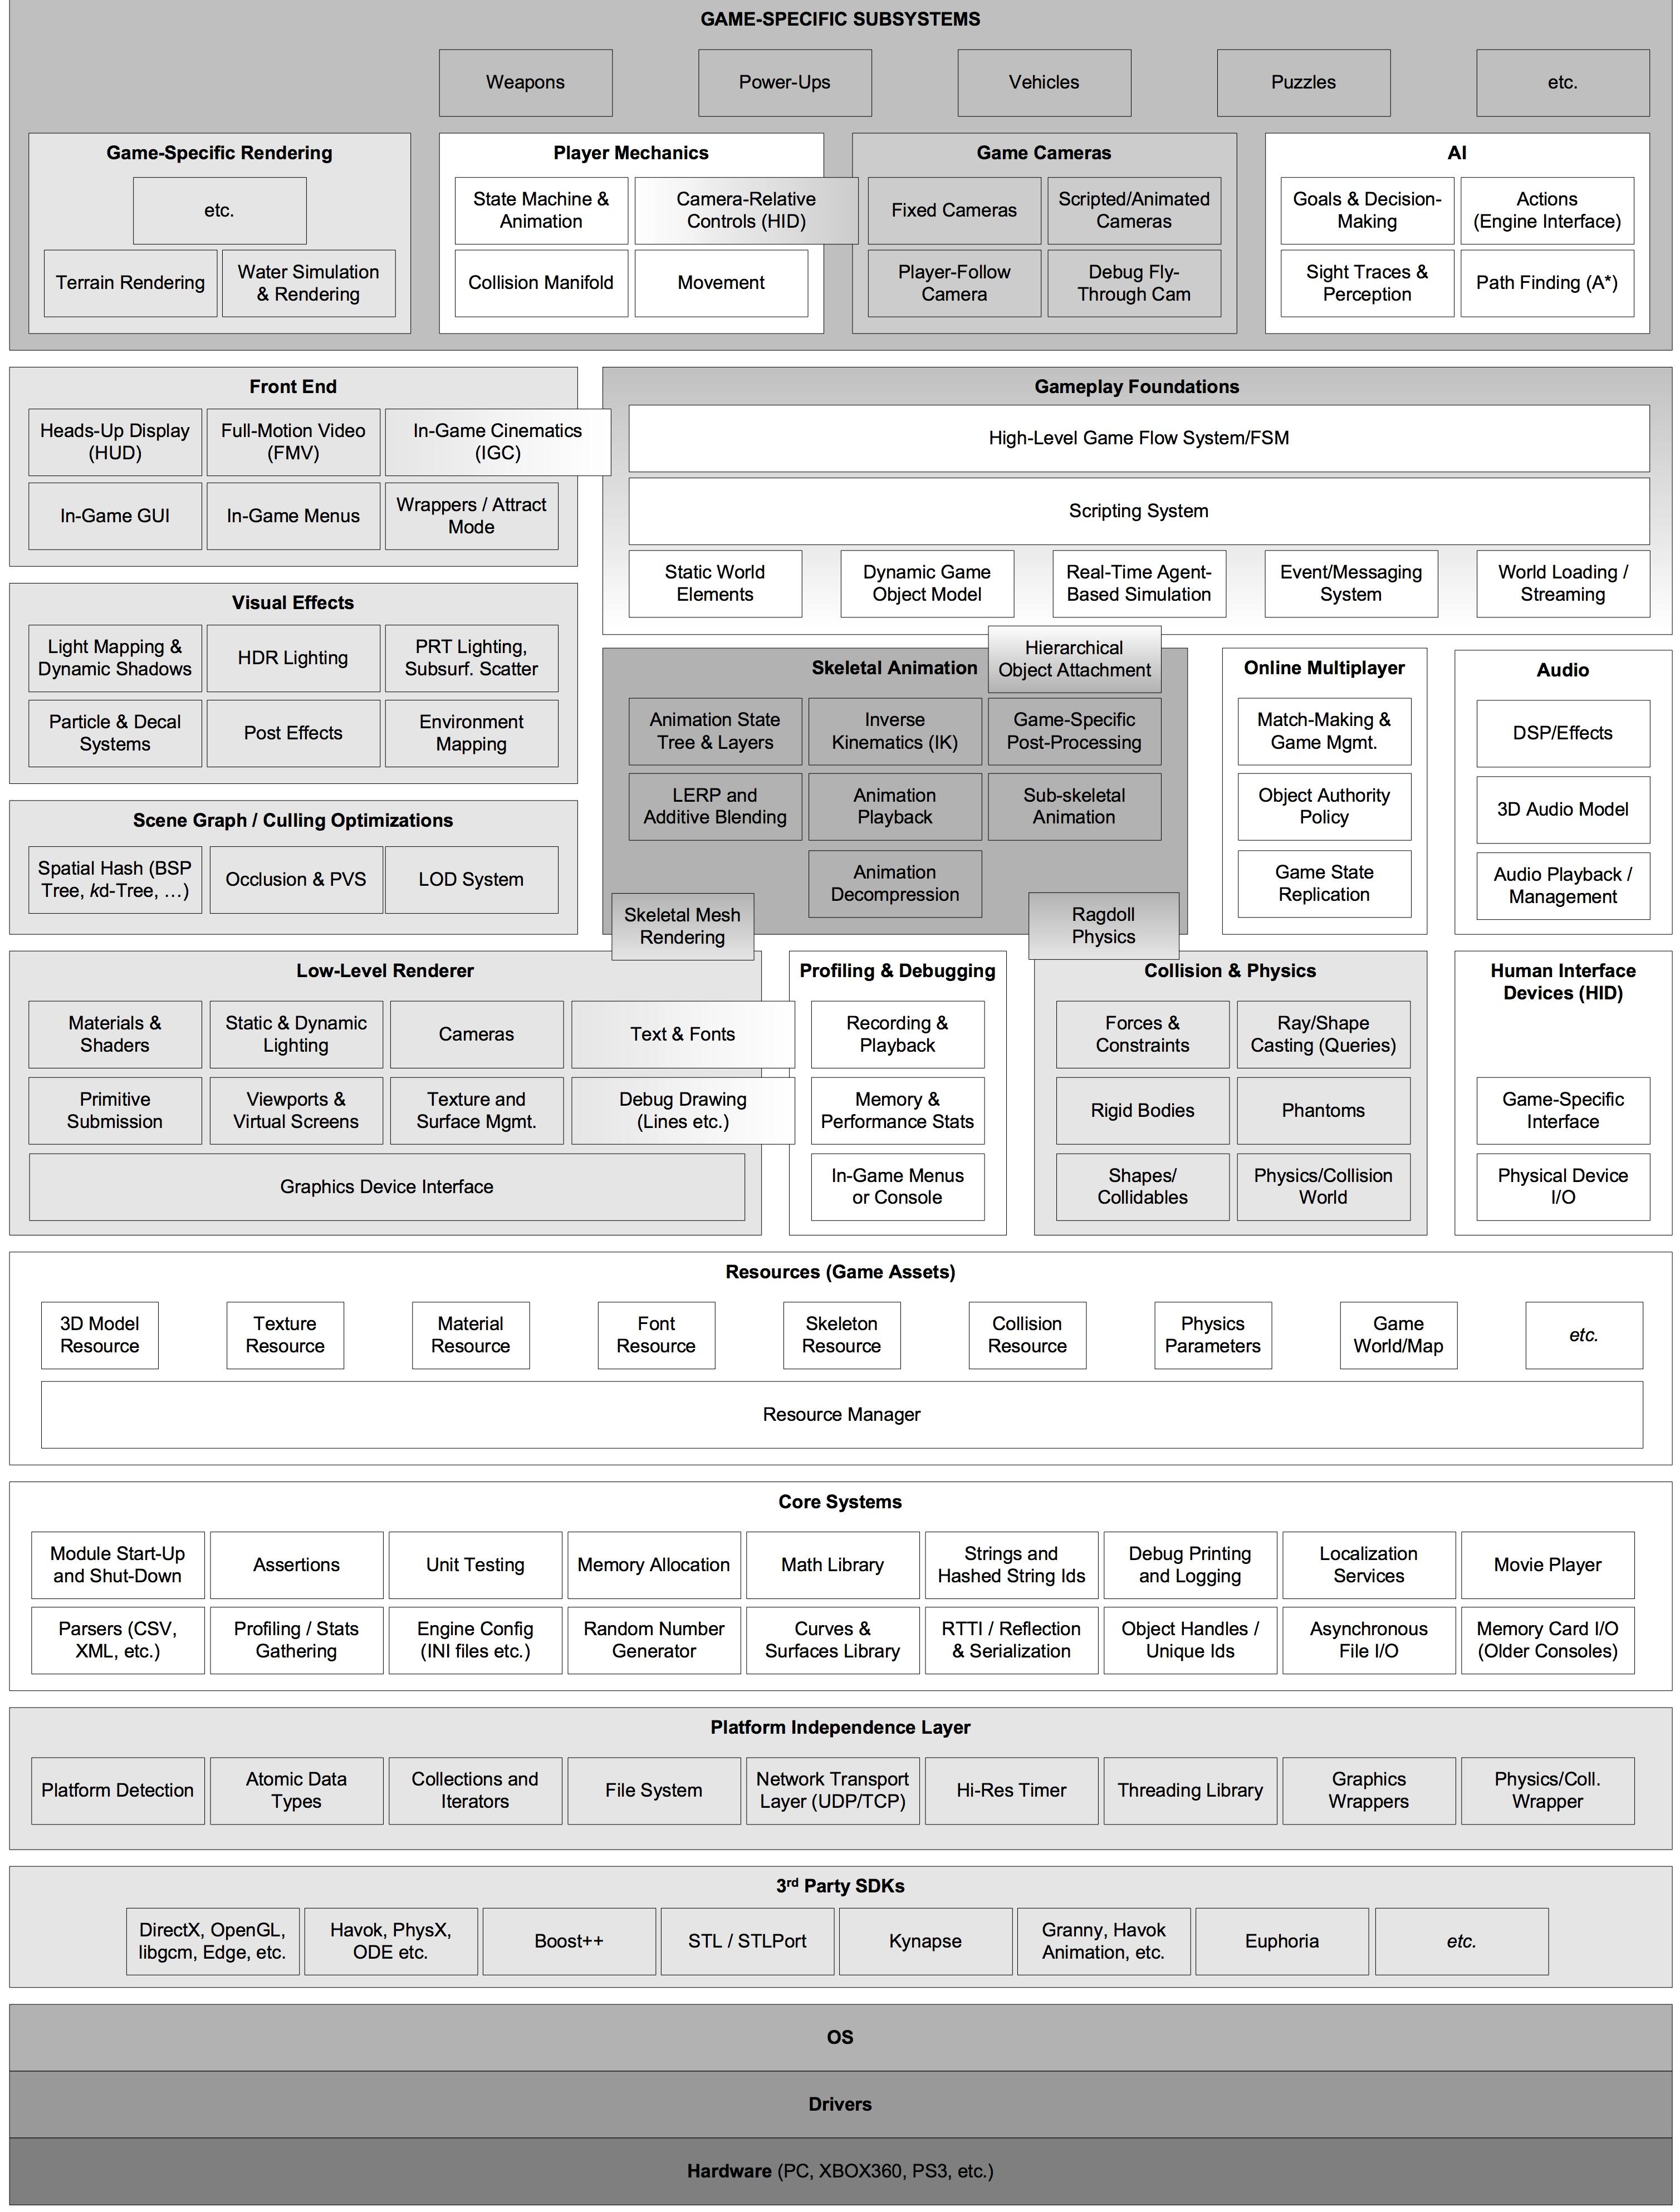
\includegraphics[width=\linewidth]{PICs/engine_runtime_arch.jpg}
	\caption{Illustration showing common modules grouped into distinct layers of a large scale engine solution}
	\label{fig:engine_runtime_arch}
\end{figure}

The complexity of modules in a layer grows when ascending through them from bottom to top. Where the lowermost layers include low-level systems essentially drivers \footnote{A program that controls or communicates with a hardware device}, platform-dependent 3\textsuperscript{rd} party \acp{SDK} or platform-independent abstraction components. Traversing the hierarchy upwards from core systems, over resource management, to general rendering and gameplay foundation modules, at one point the uppermost layers are reached. Those encompass game specific subsystems that can vary from one game to another. With the crude knowledge of the different layers involved in an engine it can be emphasized that a game engine is a highly complex software and building one is an endeavor that requires expertise, experience and time. It is important to properly reason out the architecture and uphold the focus onto the engine's goal. Maintaining focus while following the sketched out architecture will help to avoid unnecessary coupling and the implementation of irrelevant features or systems. 
The rest of this section will describe some modules from Figure \ref{fig:engine_runtime_arch} in-depth to investigate how they work and how they contribute to the combined whole.

\section{Memory Management}

One key constraint nearly every engine has to fulfill is running games with a high frame rate. Because games are real-time simulations the time window for running gameplay logic and rendering a single frame is very limited. To complement this with discrete numbers for a game, running with 60 \ac{FPS} a slice of 16.6 ms can be used per single frame. To stay into this limits game developers came up with optimization techniques and algorithms that speed up calculations and processing. But the performance of code is not only dependent upon the efficiency of an applied algorithm but also how the program manages and uses its resources, especially memory. Controlling how an engine utilizes the \ac{RAM} is mandatory for guaranteeing high performance. The two most commonly applied memory usage optimizations are either reducing the amount of dynamic allocations at a game's runtime or allocating bigger sections of memory to store data in contiguous blocks. To solve these problems engines often implement custom memory allocators that have a better runtime performance then using the existing system allocator.

\subsection{Custom Allocators}
\blindtext

\section{Job System}
\blindtext
\section{Rendering}
\blindtext
\section{Entity Component System}
\blindtext
\section{Scripting}
\blindtext
\section{Tools}
\blindtext
\subsection{Editor}
\blindtext
\subsection{Asset pipeline}
\blindtext

% Rust
\chapter{Rust}
\blindtext
\section{Current state}
\blindtext
\section{Rust ecosystem}
\blindtext
\section{Concepts}
\blindtext
\subsection{Borrow checker}
\blindtext
\subsection{Traits}
\blindtext
\subsection{Hygienic macros}
\blindtext
\section{Pitfalls}
\blindtext
% Implementation
\chapter{Subsystem implementation}
\blindtext
\section{Spark engine architecture}
\blindtext
\section{Development environment}
\blindtext
\section{Rendering framework}
\blindtext
\section{Memory Management}
\blindtext
\subsection{API}
\blindtext
\subsection{C++ implementation}
\blindtext
\subsection{Rust implementation}
\blindtext
\section{Containers}
\blindtext
\subsection{API}
\blindtext
\subsection{C++ implementation}
\blindtext
\subsection{Rust implementation}
\blindtext
\section{Entity Component System}
\blindtext
\subsection{API}
\blindtext
\subsection{C++ implementation}
\blindtext
\subsection{Rust implementation}
\blindtext
% Result evaluation
\chapter{Measures \& Comparisons}
\blindtext
\section{Environment}
\blindtext
\section{Testcases}
\blindtext
\section{C++ performance}
\blindtext
\subsection{Memory Management}
\blindtext
\subsection{Container}
\blindtext
\subsection{Entity Component System}
\blindtext
\section{Rust performance}
\blindtext
\subsection{Memory Management}
\blindtext
\subsection{Container}
\blindtext
\subsection{Entity Component System}
\blindtext
\section{Comparison}
\blindtext
% Conclusion
\chapter{Conclusion}

%
% Hier beginnen die Verzeichnisse.
%
\clearpage
\nocite{GEA_2}
\nocite{C_Lan}
\nocite{ProRus}
\nocite{GEG_3}
\nocite{Portisch17}
\bibliographystyle{IEEEtran}
\bibliography{IEEEabrv,Literatur}
\clearpage
% Das Abbildungsverzeichnis
\listoffigures
\clearpage

% Das Tabellenverzeichnis
\listoftables
\clearpage

% Das Quellcodeverzeichnis
\listofcode
\clearpage

\phantomsection
\addcontentsline{toc}{chapter}{\listacroname}
\chapter*{\listacroname}
\begin{acronym}[]
	\acro{ECS}{Entity Component System}
	\acro{GB}{Gigabyte}
	\acro{RAM}{Random-Access-Memory}
	\acro{GPU}{graphics processing unit}
	\acro{FPS}{first person shooter}
	\acro{RTS}{real-time strategy}
	\acro{UE4}{Unreal Engine 4}
	\acro{UI}{user interface}
	\acro{UBT}{Unreal Build Tool}
	\acro{UHT}{Unreal Header Tool}
	\acro{OpenGEX}{Open Game Engine Exchange Format}
	\acro{OpenDDL}{Open Data Description Language}
	\acro{IDE}{integrated development environment}
	\acro{API}{application programming interface}
	\acro{SDK}{software development kit}
	\acro{FPS}{frames per second}
\end{acronym}

\end{document}